\documentclass[12pt,a4paper]{report}
\usepackage{graphicx}
\usepackage{tabularx}
\usepackage{array}
\usepackage{geometry}
\usepackage{longtable}
\usepackage{fancyhdr}
\usepackage{sectsty}
\usepackage{blindtext}
\usepackage{listings}
\chapternumberfont{\large}
%\pagestyle{fancy}
%\lhead{Syed Hashir Husnain 2021-CS-1}
%\rhead{}
%\renewcommand{\headrulewidth}{0.4pt}
%renewcommand{\footrulewidth}{0.4pt}
\geometry{
 a4paper,
 total={210mm,297mm},
 left=19mm,
 top=19mm,
 bottom=19mm,
 right=19mm
 }

\begin{document}

\begin{center}
\thispagestyle{empty}
	%---Title---
	\vspace{2cm}
	\textbf {\huge Database System (CS-262)}\\
	\vspace {0.5cm}
	\textbf{\Large Assignment}\\
	\vspace{1cm}
	
	%---UET Logo---
	
\includegraphics[scale=0.2]{cslogo}\\
	
	%---Session---
	\vspace{1cm}
	\textit{\Large {Session 2021-2025}}\\
	\vspace{2cm}
	%---Submitted BY---
	\vspace{1cm}
	\textbf{\LARGE Submitted By}\\
	\vspace{0.5cm}
	\Large {Syed Hashir Husnain \hspace{1cm} 2021-CS-01}
	\\
	
	%---Submitted To---
	\vspace{2cm}
	\textbf{\LARGE Submitted To}\\
	\vspace{0.5cm}
	\Large Mr. Nauman Babar
	
	%---CS&UET---
	\vspace{2cm}	
	\LARGE Department of Computer Science\\
	\vspace{0.5cm}
	\textbf{\LARGE University of Engineering and Technology} \\
	\textbf{Lahore, Pakistan}	
\end{center}

%-------------------------------------------------New Page------------------------------------------------
\newpage
\thispagestyle{empty}
%---------------------------------------------Table Of Contents-------------------------------------------
\tableofcontents

\pagenumbering{arabic}

\newpage
\setcounter{page}{1}
\chapter{Assignment Report}
\section{Abstract}
The purpose of this Assignment is to practice GROUP BY and HAVING Clause concepts in Database Systems. We had given the queries related to some data. The problem is we have to filter out some data based on some conditions. DBMS helps us to do this. Just we have to write queries(means tell it) and it will generate our required output. We practiced some aggregate functions available in T-Sql and aliased the tables and columns for our simplicity. Main idea behind this assignment is to practice these queries.
\section{Technlogy Stack}
\begin{longtable}{lr} 
 \caption{Details of technology used in completion this assignment}\\
\begin{tabular}{ | m{6cm} | m{6cm}| } 
	\hline	
	\textbf{Technology} & \textbf{Version} \\ \hline
	MS SQL Server & 2022 Developer \\ \hline
	SQL Server Management Studio & 19.0.20179.0+4bc80247 \\ \hline
	Microsoft .NET Framework & 4.0.30319.42000 \\ \hline

\end{tabular}
\end{longtable}
\section{Database Schema Used}
\begin{itemize}
	\item Northwind Schema
\end{itemize}
\section{Learning Objectives}
\begin{itemize}
	\item Aggregate Functions
	\item GROUP BY Clause
	\item HAVING Clause
	\item Aliasing Method(Tables and Columns)
\end{itemize}
%-----------------------------------------NEW PAGE--------------------------------------
\newpage

\section{Lab Tasks}
%------------------------Query Template-------------------------
\subsection{Problem 01}
Perform all the group function on Northwind Schema
\subsubsection{Problem Statement}
List the total price of each category present in a stock.
\subsubsection{Query}
\begin{center}
	\begin{minipage}{12cm}
		\textbf{SELECT} CategoryID, SUM(UnitPrice) AS CategoryStockPrice\\
		\textbf{FROM} Products\\
		\textbf{GROUP BY} CategoryID
	\end{minipage}
	\begin{figure}[h]
	\centering
		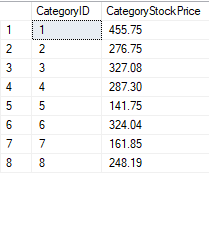
\includegraphics[scale=0.7]{images/1.png}
		\caption{Result generated: Total Price of each Category}
	\end{figure}
\end{center}

%------------------------Query Template-------------------------
\subsubsection{Problem Statement}
List the no. of products supplied by supplier in each category.
\subsubsection{Query}
\begin{center}
	\begin{minipage}{12cm}
		\textbf{SELECT} CategoryID, SupplierID, COUNT(*) AS ProductCount\\
		\textbf{FROM} Products\\
		\textbf{WHERE} UnitsOnOrder IS NOT NULL\\
		\textbf{GROUP BY} CategoryID, SupplierID
	\end{minipage}
	\begin{figure}[h]
	\centering
		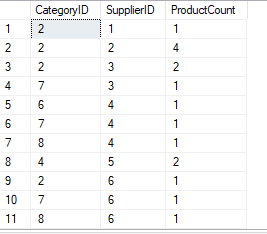
\includegraphics[scale=0.7]{images/2.png}
		\caption{Result generated: Count of Products}
	\end{figure}
\end{center}
\newpage
%------------------------Query Template-------------------------
\subsubsection{Problem Statement}
Group By can also be used as DISTINCT.
\subsubsection{Query}
\begin{center}
	\begin{minipage}{12cm}
		\textbf{SELECT} TitleOfCourtesy\\
		\textbf{FROM} Employees\\
		\textbf{GROUP BY} TitleOfCourtesy
	\end{minipage}
	\begin{figure}[h]
	\centering
		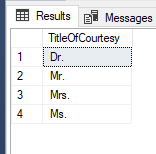
\includegraphics[scale=1]{images/3.png}
		\caption{Result generated: Alternate to DISTINCT}
	\end{figure}
\end{center}

%------------------------Query Template-------------------------
\subsection{Problem 02}
Perform all the group function using HAVING clause on Northwind Schema
\subsubsection{Problem Statement}
Select all Order IDs and their total amount where discount greater than 5 percent is applied.
\subsubsection{Query}
\begin{center}
	\begin{minipage}{12cm}
		\textbf{SELECT} OrderID, SUM(UnitPrice $*$ Quantity) TotalPrice \\
		\textbf{FROM} Order Details\\
		\textbf{GROUP BY} OrderID \\
		\textbf{HAVING} SUM(Discount) $>$ 0.5 
	\end{minipage}
	\begin{figure}[h]
	\centering
		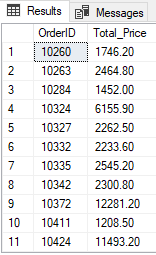
\includegraphics[scale=0.7]{images/4.png}
		\caption{Result generated: Total Price of each order}
	\end{figure}
\end{center}

%------------------------Query Template-------------------------
\newpage
\subsubsection{Problem Statement}
Select Countries which have more than one suppliers.
\subsubsection{Query}
\begin{center}
	\begin{minipage}{12cm}
		\textbf{SELECT} Country\\
		\textbf{FROM} Suppliers\\
		\textbf{GROUP BY} Country \\
		\textbf{HAVING} COUNT(ContactName)$ >$= 2
	\end{minipage}
	\begin{figure}[h]
	\centering
		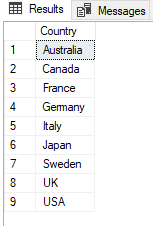
\includegraphics[scale=1]{images/5.png}
		\caption{Result generated: Multiple Suppliers}
	\end{figure}
\end{center}

%------------------------Query Template-------------------------
\subsection{Problem 03}
Apply aliasing syntax on arbitrary column on Northwind Schema.
\subsubsection{Problem Statement}
List All the customers who have ordered something.
\subsubsection{Query}
\begin{center}
	\begin{minipage}{12cm}
		\textbf{SELECT} C.ContactName AS CustomerName \\
		\textbf{FROM}  Customers AS C\\
		\textbf{JOIN} Orders AS O \\
		\textbf{ON} O.CustomerID = C.CustomerID
	\end{minipage}
	\begin{figure}[h]
	\centering
		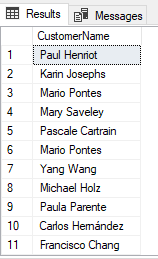
\includegraphics[scale=0.7]{images/6.png}
		\caption{Result generated: Customer Names From Orders List}
	\end{figure}
\end{center}

%------------------------------HOME TASK----------------------------------
\section{Home Tasks}
%------------------------Query Template-------------------------
\subsection{Problem 01}
\subsubsection{Problem Statement}
List name of all the products whose price is above average. 
\subsubsection{Query}
\begin{center}
	\begin{minipage}{12cm}
		\textbf{SELECT} ProductName \\
		\textbf{FROM} Products\\
		\textbf{WHERE} UnitPrice $>$ (SELECT AVG(UnitPrice) FROM Products) 
	\end{minipage}
	\begin{figure}[h]
	\centering
		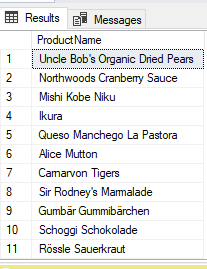
\includegraphics[scale=0.7]{images/7.png}
		\caption{Result generated: Price greater than average}
	\end{figure}
\end{center}

%------------------------Query Template-------------------------
\subsection{Problem 02}
\subsubsection{Problem Statement}
Write a query to generate report showing date wise orders shipped 
\subsubsection{Query}
\begin{center}
	\begin{minipage}{12cm}
		\textbf{SELECT} * \\
		\textbf{FROM} Orders\\
		\textbf{WHERE} ShippedDate is NOT NULL\\
		\textbf{ORDER BY} ShippedDate 
	\end{minipage}
	\begin{figure}[h]
	\centering
		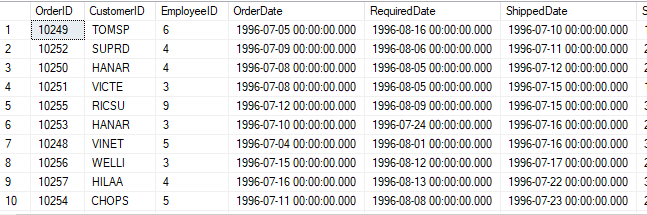
\includegraphics[scale=0.7]{images/8.png}
		\caption{Result generated: Date Wise Orders Shipped}
	\end{figure}
\end{center}


%------------------------Query Template-------------------------
\subsection{Problem 03}
\subsubsection{Problem Statement}
List name of all countries from where two or more suppliers belong to.
\subsubsection{Query}
\begin{center}
	\begin{minipage}{12cm}
		\textbf{SELECT} Country\\
		\textbf{FROM} Suppliers\\
		\textbf{GROUP BY} Country \\
		\textbf{HAVING} COUNT(ContactName) $>$= 2
	\end{minipage}
	\begin{figure}[h]
	\centering
		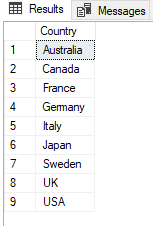
\includegraphics[scale=0.7]{images/5.png}
		\caption{Result generated: Date Wise Orders Shipped}
	\end{figure}
\end{center}

%------------------------Query Template-------------------------
\subsection{Problem 04}
\subsubsection{Problem Statement}
Write a query to generate report showing month wise orders delayed shipped.
\subsubsection{Query}
\begin{center}
	\begin{minipage}{12cm}
		\textbf{SELECT} MONTH(ShippedDate) AS MONTH, COUNT(OrderID) AS DELAYED\\
		\textbf{FROM} Orders\\
		\textbf{WHERE} RequiredDate < ShippedDate\\
		\textbf{GROUP BY} MONTH(ShippedDate)
	\end{minipage}
	\begin{figure}[h]
	\centering
		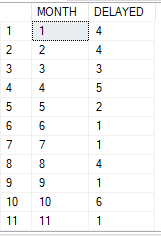
\includegraphics[scale=0.7]{images/9.png}
		\caption{Result generated: Month Wise Delayed Orders}
	\end{figure}
\end{center}

%------------------------Query Template-------------------------
\subsection{Problem 05}
\subsubsection{Problem Statement}
Report all the orders which have been discounted. Your result should show the total discount against each 
order.
\subsubsection{Query}
\begin{center}
	\begin{minipage}{12cm}
		\textbf{SELECT} OrderID, SUM(Discount) AS  DISCOUNT\\
		\textbf{FROM} Order Details\\
		\textbf{GROUP BY} OrderID\\
		\textbf{HAVING} SUM(Discount) $<>$ 0
	\end{minipage}
	\begin{figure}[h]
	\centering
		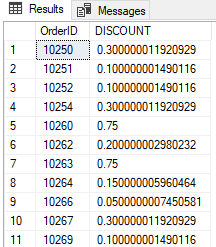
\includegraphics[scale=0.7]{images/10.png}
		\caption{Result generated: Discounted Orders}
	\end{figure}
\end{center}

%------------------------Query Template-------------------------
\subsection{Problem 06}
\subsubsection{Problem Statement}
Write a query to list the number of orders which were shipped in the cities of USA in 1997. Show the 
number of order against each city. 
\subsubsection{Query}
\begin{center}
	\begin{minipage}{12cm}
		\textbf{SELECT} ShipCity, COUNT(OrderID) Orders\_IN\_USA\_IN\_1997\\
		\textbf{FROM} Orders\\
		\textbf{WHERE} ShipCountry = 'USA' AND YEAR(ShippedDate) = 1997\\
		\textbf{GROUP BY} ShipCity
	\end{minipage}
	\begin{figure}[h]
	\centering
		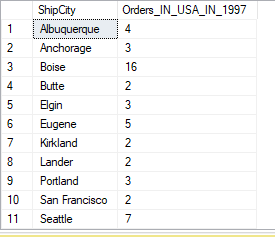
\includegraphics[scale=0.7]{images/11.png}
		\caption{Result generated: Orders Shipped in Cities of USA}
	\end{figure}
\end{center}

%------------------------Query Template-------------------------
\subsection{Problem 07}
\subsubsection{Problem Statement}
Write a query to generate report showing country wise orders delayed shipped. 
\subsubsection{Query}
\begin{center}
	\begin{minipage}{12cm}
		\textbf{SELECT} ShipCountry, COUNT(OrderID) AS Orders\_Delayed\\
		\textbf{FROM} Orders\\
		\textbf{WHERE} RequiredDate $<$ ShippedDate\\
		\textbf{GROUP BY} ShipCountry
	\end{minipage}
	\begin{figure}[h]
	\centering
		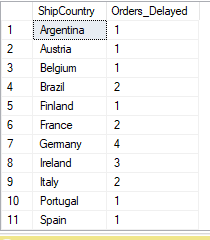
\includegraphics[scale=0.7]{images/12.png}
		\caption{Result generated: Orders Delayed Country Wise}
	\end{figure}
\end{center}

%------------------------Query Template-------------------------
\subsection{Problem 08}
\subsubsection{Problem Statement}
Report all the orders which have been discounted with total price of order. Your result should show the 
total discount against each order.
\subsubsection{Query}
\begin{center}
	\begin{minipage}{15cm}
		\textbf{SELECT} OrderID, SUM(Discount) AS DISCOUNT, SUM(((100-Discount )/100)*UnitPrice) AS TotalPrice\\
		\textbf{FROM} Order Details\\
		\textbf{GROUP BY} OrderID\\
		\textbf{HAVING} SUM(Discount) $<>$ 0
	\end{minipage}
	\begin{figure}[h]
	\centering
		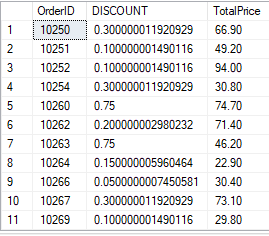
\includegraphics[scale=0.7]{images/13.png}
		\caption{Result generated: Discounted Orders with Total Price}
	\end{figure}
\end{center}

%------------------------Query Template-------------------------
\subsection{Problem 09}
\subsubsection{Problem Statement}
Write a query to list the number of orders which were shipped in the cities of each region in 1997. Show 
the number of order against each city.
\subsubsection{Query}
\begin{center}
	\begin{minipage}{13cm}
		\textbf{SELECT} ShipRegion, ShipCountry, COUNT(OrderID) AS Orders\\
		\textbf{FROM} Orders\\
		\textbf{WHERE} ShipRegion IS NOT NULL AND YEAR(ShippedDate) = 1997\\
		\textbf{GROUP BY} ShipRegion, ShipCountry
	\end{minipage}
	\begin{figure}[h]
	\centering
		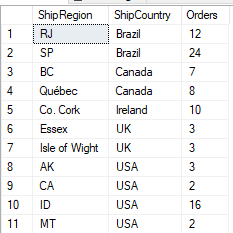
\includegraphics[scale=0.7]{images/14.png}
		\caption{Result generated: Orders Shipped in each region}
	\end{figure}
\end{center}

\end{document}
